\documentclass[twoside, final]{hcmut_report}
\usepackage{codespace}
% Configuration
\upperuniname{ĐẠI HỌC QUỐC GIA THÀNH PHỐ HỒ CHÍ MINH}
\uniname{TRƯỜNG ĐẠI HỌC BÁCH KHOA}
\deptname{KHOA KHOA HỌC VÀ KỸ THUẬT MÁY TÍNH}

\coursename{XÁC SUẤT VÀ THỐNG KÊ}
\reporttype{BÁO CÁO BÀI TẬP LỚN}
\title{PHÂN TÍCH BỘ DỮ LIỆU VỀ SẢN PHẨM CỦA CỬA HÀNG ĐIỆN TỬ ONLINE}
\advisor{
    TS. Phan Thị Hường
}
\student{
    Trần Điền Minh          ,   2312116
    Phan Thanh Sơn          ,   2312975
    Nguyễn Hoàng Anh Thắng  ,   2313185
    Huỳnh Văn Lợi           ,   2311974
    Cao Chí Nguyên          ,   2312331
    Nguyễn Hữu Thịnh        ,   2313292
}

\begin{document}
\begin{titlepage}
    \coverpage
\end{titlepage}
\newpage
\setcounter{page}{1}
\pagestyle{empty}
\tableofcontents
\pagestyle{fancy}
\pagebreak
Cách xuống dòng

bằng double enter
\section{Kiểu liệt kê}
\subsection{dấu chấm}

\begin{itemize}
    \item a 
    \item b 
    \item c 
\end{itemize}

\subsection{chữ số}
\begin{enumerate}
    \item a 
    \item b 
    \item c
\end{enumerate}

\section{Công thức toán}
$a^2+b^2=c^2$
$$a^2+b^2=c^2$$

\section{Chèn hình}
\begin{figure}[!htbp]
    \centering
    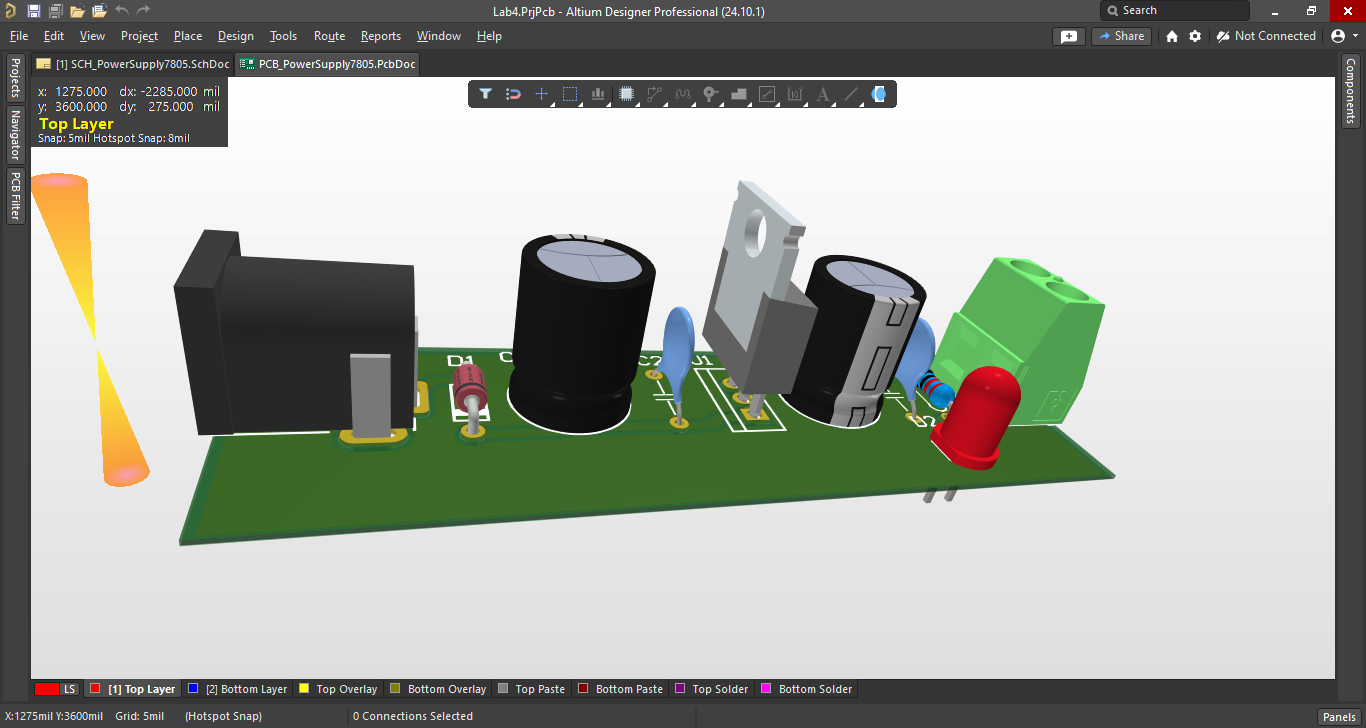
\includegraphics[width=0.7\textwidth]{graphics/f5.PNG}
    \caption{3D PCB}
\end{figure}

\section{Chèn code}
\begin{lstlisting}
    assump_data <- data.frame(Max_Power_Value = 225, Memory_Value = 8190, Memory_Bandwidth_Value = 70)
    predict(mo.hinh.3, assump_data, interval = "confidence")
\end{lstlisting}
\end{document}